This section details the analysis and statistical exploration of the extracted \textbf{Elevation Dataset} for the combined region of Algeria and Tunisia. The dataset is examined for data integrity, statistical properties, and spatial distribution.

\subsection{Data Loading and Integrity Check}

The analysis begins by loading the processed raster file using \texttt{rasterio}.

\begin{itemize}
    \item \textbf{No-Data Handling:} An integrity check was performed to identify and quantify the raster's no-data values (\texttt{nodata\_value}). These values, often representing areas outside the clipped boundary or sea level, were masked out during statistical calculations to ensure accurate topographical analysis.
\end{itemize}


\subsection{Descriptive Statistics and Visualisation}

Core statistics were computed on the valid elevation pixels to characterize the overall terrain:
    
    \begin{itemize}
        \item Mean Elevation: 538.327
        \item Median Elevation: 464.0
        \item Mode Elevation: 301
    \end{itemize}

The \textbf{Elevation Dataset}  was visualized to create a professional elevation map. The map utilizes a color scale to intuitively display elevation in meters.
 
\begin{figure}[H]
    \centering
    % Placeholder for the Elevation Map visualization
    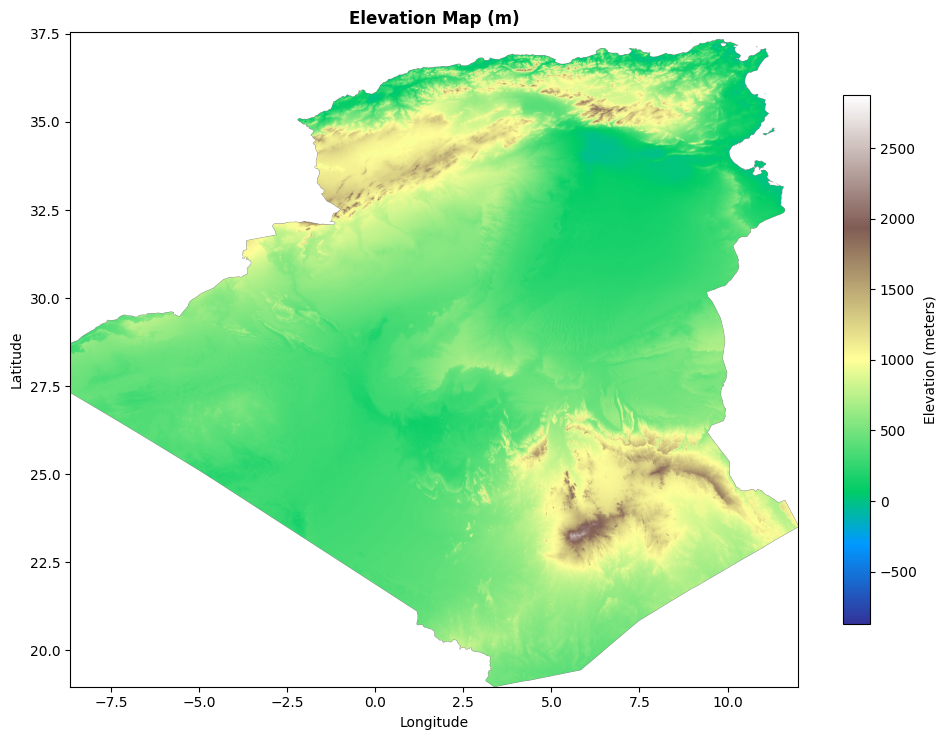
\includegraphics[width=0.5\textwidth]{images/Elevation/elevation map.png}
    \caption{Color-ramped visualization of the Elevation Dataset for the combined Algeria and Tunisia study area. The \texttt{terrain} color map illustrates the topographical gradient, ranging from low coastal plains to high inland mountains.}%
    \label{fig:elevation_map}
\end{figure}
